\chapter{Воздушные суда от мала до велика}%
\label{ch:aircraft-chapter}

Глава посвящена исследованию различных свойств воздушных судов 
на основе базы знаний международного проекта Викиданные. 
В ходе исследования с помощью SPARQL-запросов, вычисляемых на объектах типа <<Воздушные суда>> в Викиданных, 
получены сведения о всех воздушных судах и их произведённом количестве, 
также получена диаграмма соотношения количества производителей воздушных судов по странам. 
В заключении работы дана оценка полноты данных, представленных в Википедии и Викиданных.

Авиационная промышленность является одной из самой крупнейшей отраслью машиностроения в мире. 
В её задачи входит как разработка так и производство различной воздушной техники. 
Для того чтобы оценить, какие модели воздушных судов являются самыми массовыми, 
мы построим диаграмму по количеству выпущенных судов различных моделей.

На рисунке рис.~\ref{fig:Number_of_aircraft_produced_ru_2020} видно, что на 2020 год больше всего было выпущено воздушных судов следующих моделей: Piper PA-32 (7842 штук), Piper PA-24 Comanche (4857), Junkers W 34 (3000), Piper J-4 (1251).

%\begin{figure}[h]
%\centering
%	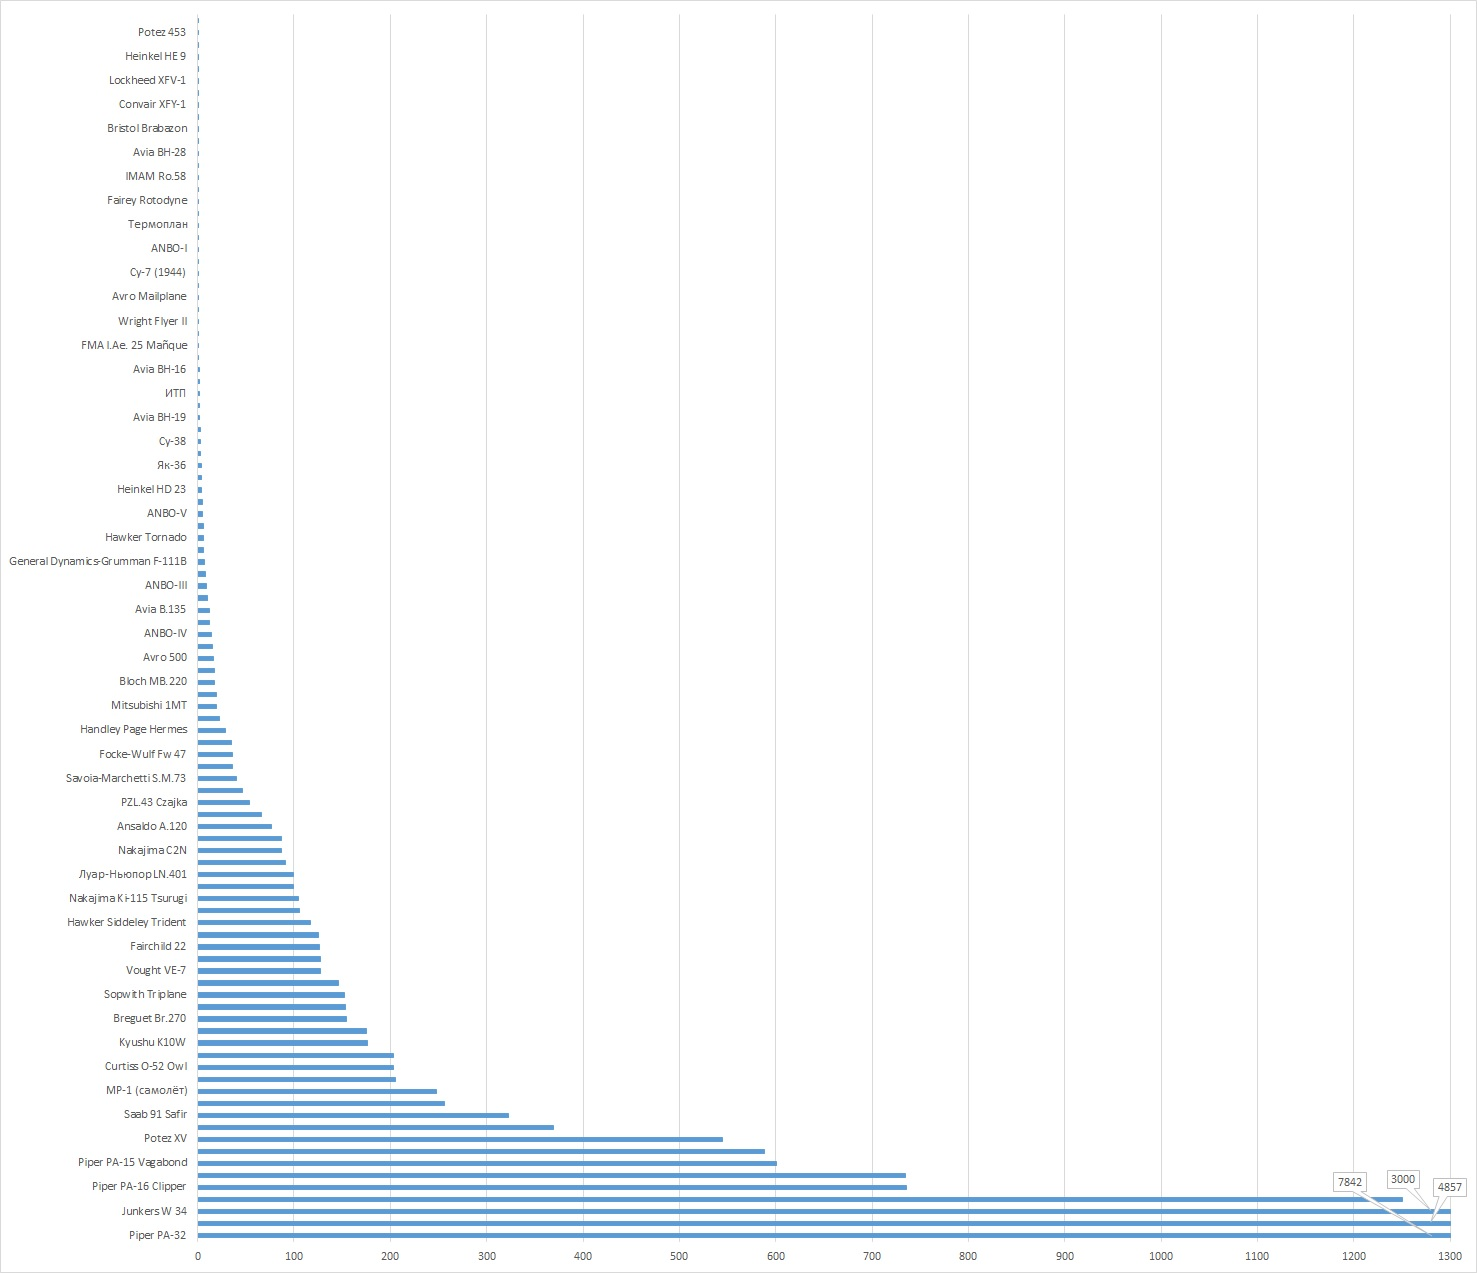
\includegraphics[width=0.7\textwidth]{./chapter/aircraft/Number_of_aircraft_produced_ru.jpg}
%	\caption{Количество выпущенных воздушных судов по моделям, 2020.}
%	\label{fig:Number_of_aircraft_produced_ru_2020}
%\end{figure}

\clearpage
\begin{figure*}[h]

    \setlength{\fboxsep}{0pt}%
    \setlength{\fboxrule}{1pt}%
    \fcolorbox{gray}{gray}{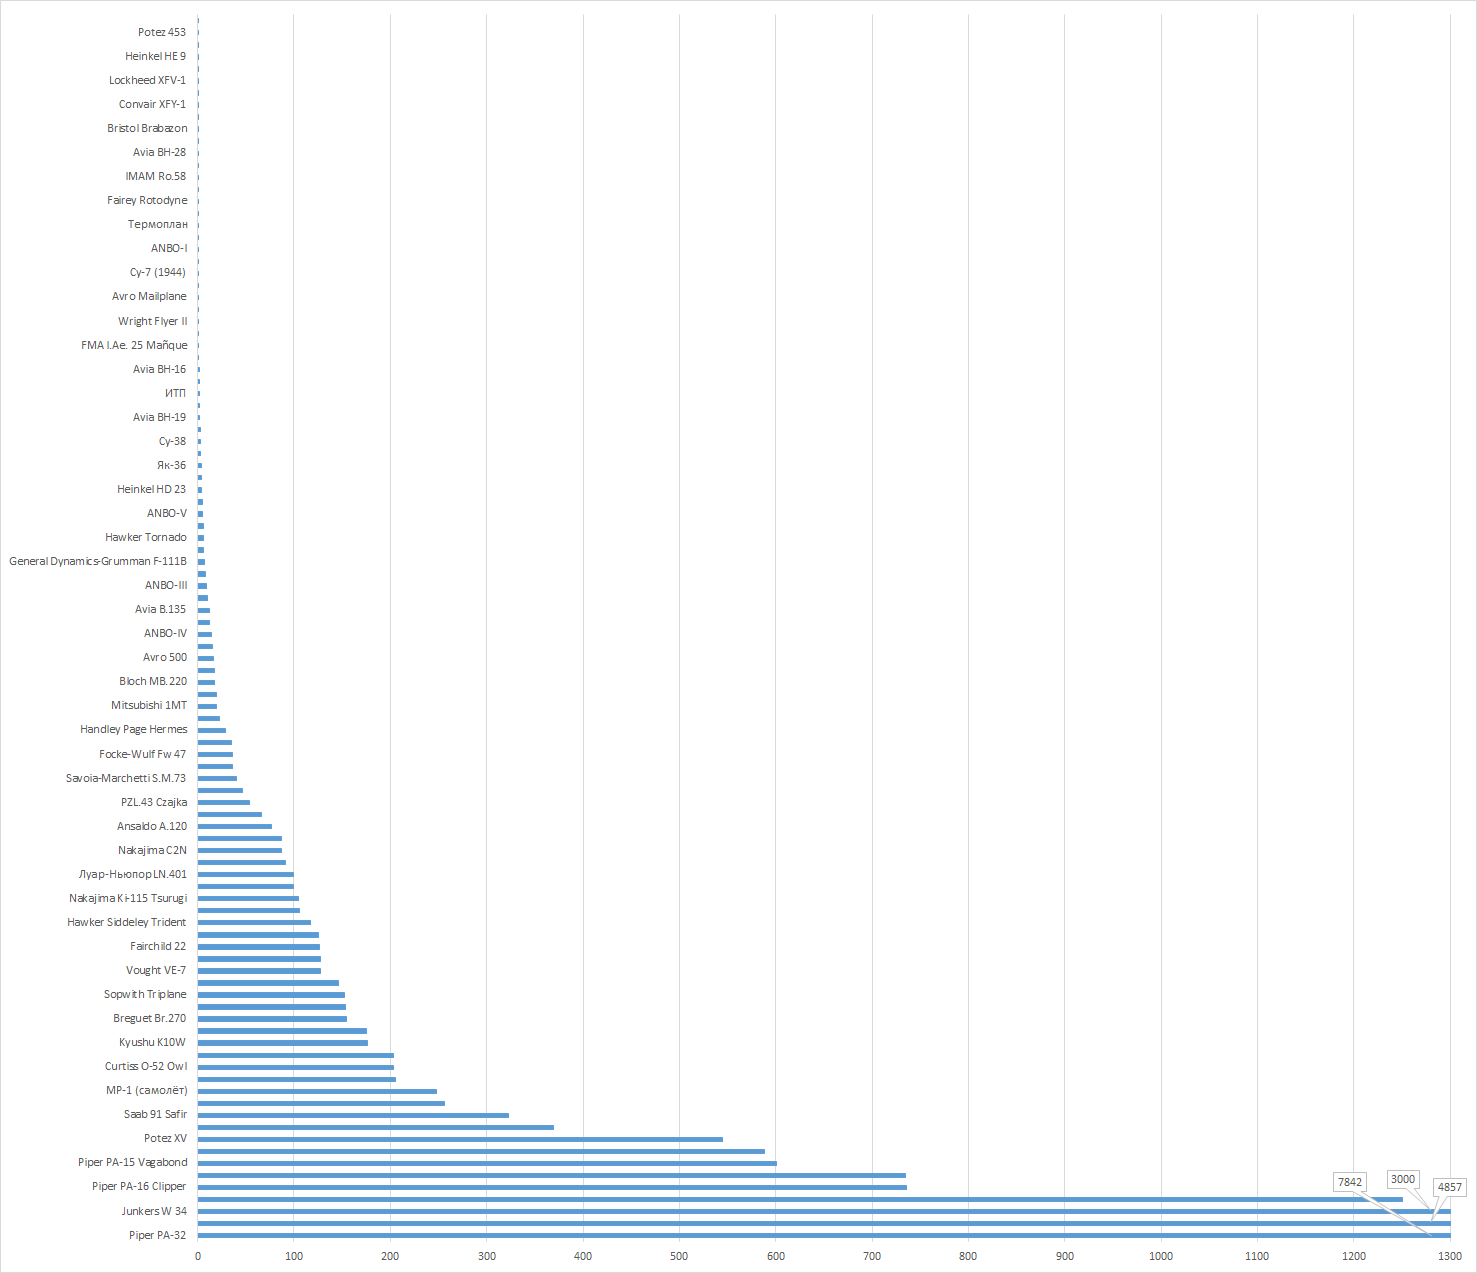
\includegraphics[width=\linewidth]{./chapter/aircraft/Number_of_aircraft_produced_ru.png}}%

%	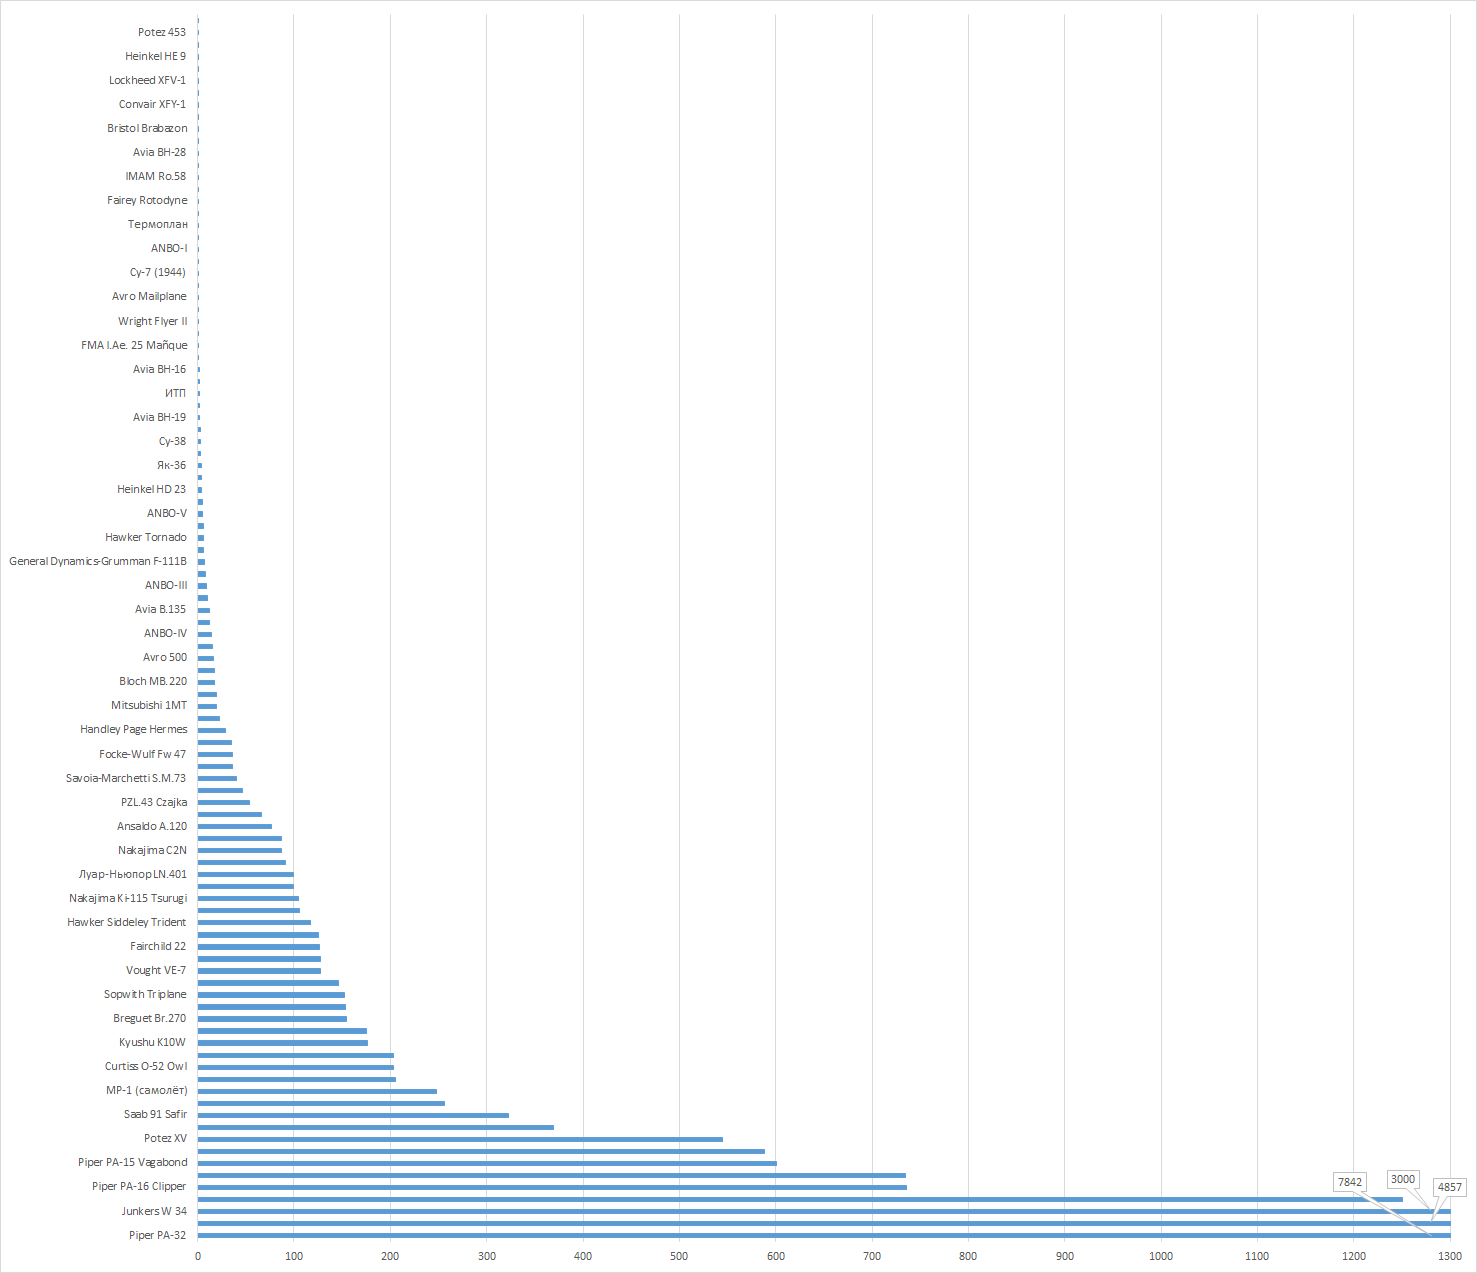
\includegraphics{./chapter/aircraft/Number_of_aircraft_produced_ru.png}%
	\caption{Количество выпущенных воздушных судов по моделям, 2020.}%
    \label{fig:Number_of_aircraft_produced_ru_2020}%
\end{figure*}

Исходя из полученных данных можно подсчитать, что всего было произведено 24927 единиц воздушной техники.
